% Dua pasar: rumah menengah ke atas (peduli iklim) dan B2B multi-turbin.
\documentclass[border=4pt]{standalone}
% Gaya bersama gambar deck Demo Day (dipakai semua gambar/*.tex standalone).
\usepackage{amssymb}
\usepackage{fontspec}
\setmainfont{DejaVu Sans Condensed}
\setsansfont{DejaVu Sans Condensed}
\newfontfamily\judulfont{DejaVu Sans}[BoldFont={DejaVu Sans Bold}, Ligatures=TeX]
\usepackage{tikz,pgfplots}
\pgfplotsset{compat=1.18, every axis/.append style={/pgf/number format/assume math mode=true, /pgf/number format/use comma, /pgf/number format/1000 sep={.}}}
\usetikzlibrary{positioning,arrows.meta,calc,shapes.geometric,fit,backgrounds}
\definecolor{gelap}{HTML}{15242B}
\definecolor{teal}{HTML}{285052}
\definecolor{amber}{HTML}{E8A317}
\definecolor{muda}{HTML}{DCE8E8}
\definecolor{abu}{HTML}{8A9499}
\definecolor{teks}{HTML}{1E2B30}
\definecolor{hijau}{HTML}{2F7D5B}
\definecolor{merah}{HTML}{A33A2A}
\color{teks}
\tikzset{
  ubin/.style={fill=muda, rounded corners=5pt, align=center, inner sep=6pt},
  inti/.style={ubin, fill=gelap, text=white},
  panah/.style={-{Stealth[length=3mm]}, line width=1.3pt, draw=amber},
  panahabu/.style={-{Stealth[length=2.5mm]}, line width=1pt, draw=abu},
  judulubin/.style={font=\judulfont\bfseries},
}
% Dibuat otomatis oleh buat_aset.py dari ml/results/energi_harian.json; jangan diedit manual.
\newcommand{\energiTurbin}{270}
\newcommand{\energiQa}{187}
\newcommand{\energiQb}{377}
\newcommand{\hariEnergi}{140}
\newcommand{\raspiWh}{71}
\newcommand{\chipWh}{4,1}
\newcommand{\raspiPersen}{26}
\newcommand{\chipPersen}{1,5}
\newcommand{\raspiPersenA}{19}
\newcommand{\raspiPersenB}{38}
\newcommand{\raspiPersenNum}{26.3}
\newcommand{\chipPersenNum}{1.5}
\newcommand{\hematKwh}{24}
\newcommand{\kaliHemat}{17}
\newcommand{\jRaspi}{182}
\newcommand{\jChip}{10,4}
\newcommand{\periodeEnergi}{2026-03-31--2026-10-20}

\AtBeginDocument{\hyphenpenalty=10000 \exhyphenpenalty=10000}

\begin{document}
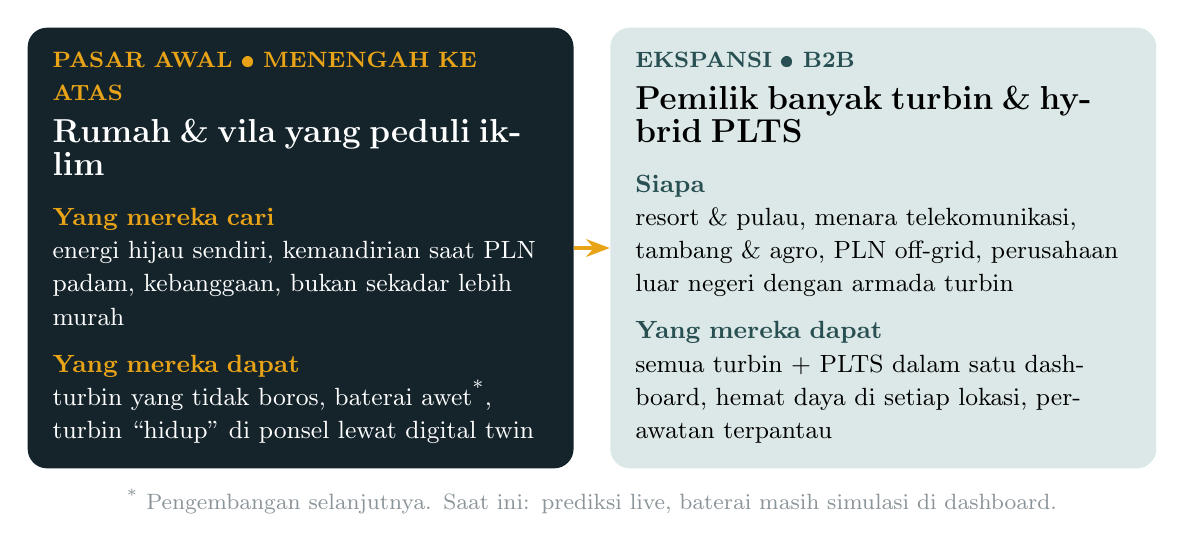
\begin{tikzpicture}[font=\fontsize{9.5}{12}\selectfont,
  persona/.style={rounded corners=7pt, text width=6.3cm, minimum height=5.45cm, align=left, inner sep=9pt, anchor=north west}]
  \node[persona, fill=gelap, text=white] (a) at (0,0) {%
    {\color{amber}\fontsize{8.5}{10}\selectfont\bfseries PASAR AWAL \textbullet{} MENENGAH KE ATAS}\\[3pt]
    {\judulfont\bfseries\fontsize{13}{15}\selectfont Rumah \& vila yang peduli iklim}\\[6pt]
    {\color{amber}\textbf{Yang mereka cari}}\\
    energi hijau sendiri, kemandirian saat PLN padam, kebanggaan, bukan sekadar lebih murah\\[5pt]
    {\color{amber}\textbf{Yang mereka dapat}}\\
    turbin yang tidak boros, baterai awet\textsuperscript{*}, turbin ``hidup'' di ponsel lewat digital twin};
  \node[persona, fill=muda] (b) at (7.4,0) {%
    {\color{teal}\fontsize{8.5}{10}\selectfont\bfseries EKSPANSI \textbullet{} B2B}\\[3pt]
    {\judulfont\bfseries\fontsize{13}{15}\selectfont Pemilik banyak turbin \& hybrid PLTS}\\[6pt]
    {\color{teal}\textbf{Siapa}}\\
    resort \& pulau, menara telekomunikasi, tambang \& agro, PLN off-grid, perusahaan luar negeri dengan armada turbin\\[5pt]
    {\color{teal}\textbf{Yang mereka dapat}}\\
    semua turbin + PLTS dalam satu dashboard, hemat daya di setiap lokasi, perawatan terpantau};
  \draw[panah] (a.east) -- (b.west);
  \node[anchor=north, text=abu, text width=13.5cm, align=center, font=\fontsize{8.5}{10}\selectfont] at ([yshift=-4pt]current bounding box.south) {\textsuperscript{*} Pengembangan selanjutnya. Saat ini: prediksi live, baterai masih simulasi di dashboard.};
\end{tikzpicture}
\end{document}
